
%----------------------------------------------------------------------------------------
%	PREAMBUŁA
%----------------------------------------------------------------------------------------

\documentclass[12pt]{article}
\usepackage[polish]{babel}
\usepackage{polski}
\usepackage[utf8]{inputenc}
%\usepackage[T1]{fontenc}
\usepackage{amsmath}
\usepackage{graphicx}
\usepackage{fancyhdr}
\usepackage{float}
\usepackage{graphicx}
\usepackage{hyperref}
\usepackage{verbatim}

\usepackage{subfig}

\usepackage{color} %red, green, blue, yellow, cyan, magenta, black, white
\definecolor{mygreen}{RGB}{28,172,0} % color values Red, Green, Blue
\definecolor{mylilas}{RGB}{170,55,241}


\title{Sprawozdanie}
\author{Aleksandra Poręba}

\graphicspath{{static/}} 

\makeatletter
\let\thetitle\@title
\let\theauthor\@author
\let\thedate\@date
\makeatother


%----------------------------------------------------------------------------------------
%	STRONA TYTUŁOWA
%----------------------------------------------------------------------------------------
\begin{document}
\begin{center}
\textsc{\normalsize Wydział Fizyki i Informatyki Stosowanej}\\[2.0cm] 

\includegraphics[scale = 1]{logo.png}\\[1cm] 
%\textsc{\Large Modelowanie Procesów Fizycznych}\\[0.4cm] 


\textsc{\Large Sprawozdanie}\\[0.4cm]
{ \huge \bfseries \LARGE{Projekt 2: Model Sznajdów 2D} }\\[1cm] 

\flushright \Large Aleksandra Poręba \\ nr. indeksu 290514

\vfill 

\center{\today}


\pagebreak 

\end{center}

%----------------------------------------------------------------------------------------
%	SPIS TREŚCI
%----------------------------------------------------------------------------------------
%\tableofcontents
%\pagebreak

%----------------------------------------------------------------------------------------
%	ZAWARTOŚĆ
%----------------------------------------------------------------------------------------

\pagestyle{fancy}
\fancyhf{}

\rhead{\theauthor}
\lhead{\thetitle}
\cfoot{\thepage}

\section{Opis projektu}

Model Sznajdów lub model ''\textit{United we stand, divided we fall}'' jest używany do modelowania formowania się opinii w społeczeństwie. Został on opracowany przez Katarzynę Sznajd-Weron oraz Józefa Sznajd.

W modelu możemy zaobserwować zachowania konformistyczne, wylosowana para osobników - spinsonów (spin + person) decyduje o opinii jej sąsiadów. Gdy para jest zgodna, opinia sąsiadów zostaje zmieniona na opinię pary. W oryginalnej wersji automatu w przypadku niezgody dwóch osobników nie obserwowano żadnych efektów w społeczeństwie. Jako rozszerzenie została dodana opcja kłócenia się - w przypadku niezgodny spinsonów ich sąsiedzi zaczynają się z nimi kłócić.

Każdy osobnik może przyjmować jedną z dwóch opini: '$+$' lub '$-$', tak lub nie, zielony lub czerwony.

\begin{figure}[H]
\centering
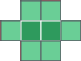
\includegraphics[width=0.2\textwidth]{zgoda.png} \qquad
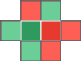
\includegraphics[width=0.2\textwidth]{nic.png} \qquad
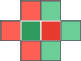
\includegraphics[width=0.2\textwidth]{klocenie.png}
\caption{Możliwe stany w zależności od opinii wylosowanej pary. Na pierwszym rysunku przedstawiona jest sytuacja, gdy wylosowana para jest zgodna - sąsiedzi przyjęli tą samą opinię. Na środkowym rysunku przedstawiony jest stan z wyłączonym kłóceniem się - opinia sąsiadów pozostaje niezmienna, a po prawej sytuacja z włączonym kłóceniem się - sąsiedzi spinsona z pary przyjmują opinie przeciwne niż spinson.}
\end{figure}

W projekcie został przedstawiony model dwuwymiarowy, każda para wpływa na opinię swoich sześciu sąsiadów ( sąsiedztwo \textit{von Neumana} ).


\section{Stany automatu}
Dojście automatu do stanu stacjonarnego zajmuje bardzo dużo czasu, szczególnie, gdy włączona jest opcja kłócenia się. Jest to spowodowane faktem, że w jednym kroku losowana jest tylko jedna para. Aby zaobserwować stan stacjonarny w skończonym czasie zaleca się ustawienie małej siatki. Zazwyczaj przeważa w nim ta opcja, której początkowo było więcej.

Możliwe jest również osiągnięcie stanu, w którym wszystkie osobniki się ze sobą kłócą - czyli wszyscy sąsiedzi osobnika mają opinię przeciwną niż osobnik. Jest on możliwy, gdy włączona jest opcja kłócenia się.

\subsection{Stany pośrednie}

Poniżej przedstawiono stan pośredni dla opcji z kłóceniem się i bez kłócenia.

\begin{figure}[H]
\centering
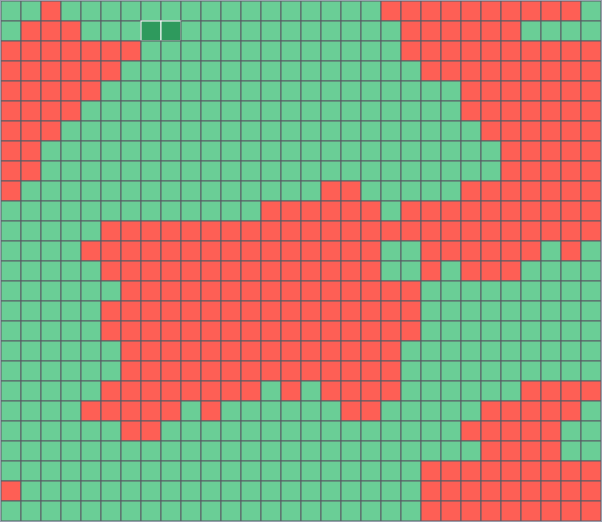
\includegraphics[width=0.4\textwidth]{sym_bez.png} \quad
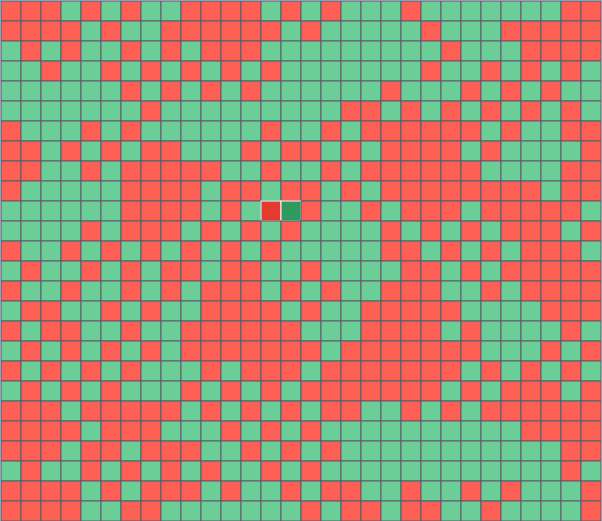
\includegraphics[width=0.4\textwidth]{sym_klocenie.png}
\caption{Powyżej przedstawione zostały stany pośrednie automatu dla dużej siatki z wyłączonym i włączonym kłóceniem się. W obu przypadkach początkowy rozkład opinii wynosił $50:50$. }
\end{figure}

Na rysunku po lewej stronie można zauważyć, że opinie połączone są w ścisłe grupy, zmiana opinii może zajść tylko na brzegach zbiorów. Gdy zostanie wylosowany element ze środka zbioru, nie zmieni to rozkładu opinii w społeczeństwie.

Po prawej, w automacie z włączonym kłóceniem się sąsiadów można zaobserwować przejścia pomiędzy zbiorami, gdzie wszyscy sąsiedzi ( z otoczenia \textit{von Neumana} ) danego osobnika mają opinię przeciwną do niego. Grupy jednolitych opinii są mniejsze niż w przypadku pierwszego rysunku. Z powodu dużych obszarów pośrednich, które mają tendencję zajmować większość siatki, jest większe prawdopodobieństwo osiągnięcia stanu, w którym wszystkie osobniki się ze sobą kłócą.

\subsection{Stan stacjonarny ''kłótnia''}

Poniżej przedstawiony został stan stacjonarny, w którym wszystkie osobniki mają opinię różną niż ich sąsiedzi. W automacie kłócenie się zostało włączone.

\begin{figure}[H]
\centering
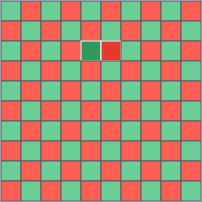
\includegraphics[width=0.25\textwidth]{stacjonarny_klocenie.png} 
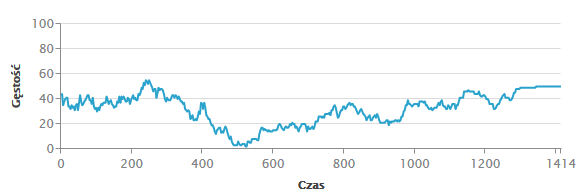
\includegraphics[width=0.7\textwidth]{stacjonarny_klocenie_wykres.png}
\caption{Jeden z możliwych stanów stacjonarnych. }
\end{figure}

Na wykresie powyżej można zauważyć, że automatowi zajęło około 1300 kroków czasowych do osiągnięcia stanu stacjonarnego. Około kroku 500 automatowi udało się go prawie osiągnąć, dla wszystkich opinii ''czerwonych'', jednak losowy charakter wyboru pary i szczęśliwy przypadek zadecydował o pojawianiu się większej ilości ''zielonych''.

\subsection{Porównanie automatu w zależności od włączonego ''kłócenia się''}

Poniżej zostały przedstawione wykresy dojścia do stanu stacjonarnego dla automatu z włączonym i wyłączonym kłóceniem się.

\begin{figure}[H]
\centering
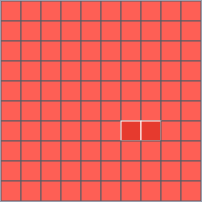
\includegraphics[width=0.3\textwidth]{stacjonarny_niezgoda.png}
\caption{Stan stacjonarny z jednolitą opinią. }
\end{figure}

\begin{figure}[H]
\centering
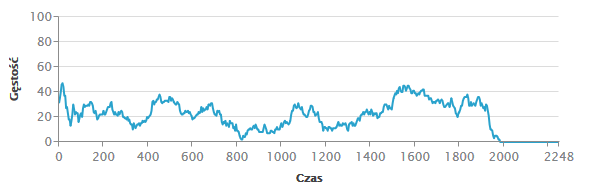
\includegraphics[width=0.7\textwidth]{stacjonarny_niezgoda_wykres.png} 
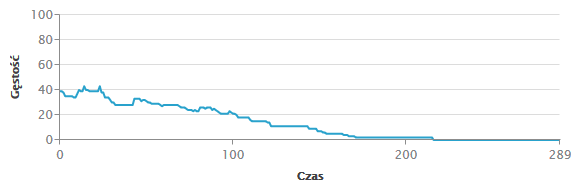
\includegraphics[width=0.7\textwidth]{stacjonarny_niezgoda_wykres_bezk.png}
\caption{Wykresy przedstawiające gęstość ''zielonych'' w kolejnych krokach czasowych.}
\end{figure}

Automatowi bez ''kłócenia się'' osiągnięcie stanu zajęło około 170 kroków czasowych. Krzywa jest raczej gładka.

W przypadku włączonej opcji kłócenia przebieg wykresu jest bardziej dynamiczny. Około kroku $800$ prawie został osiągnięty stan stacjonarny (tylko ''czerwoni''), podobnie w okolicach kroku $1600$ (stan ''wszyscy się ze sobą kłócą''). Finalnie, po kroku $2000$ został osiągnięty stan z wszystkimi czerwonymi osobnikami. Temu automatowi osiągnięcie stanu stacjonarnego zajęło 10 razy dłużej niż opcji z wyłączonymi kłótniami.

\section{Obsługa aplikacji}
W aplikacji możliwa jest modyfikacja początkowej gęstości ''zielonych'' na siatce oraz jej rozmiaru za pomocą z menu ''Parametry wejściowe''. Najmniejsza możliwa siatka to $10$ x $10$, największa zależy od aktualnej wielkości okna. Również w menu można wybrać, czy w przypadku niezgody pary ich sąsiedzi mają zacząć się z nimi kłócić, czy pozostać niezmienni.

Poniżej menu znajduje się wykres prezentujący gęstości ''zielonych'' w społeczeństwie dla kolejnych iteracji. Po prawej stronie aplikacji znajduje się siatka, na której prezentowane jest działanie automatu.

Symulacją można sterować za pomocą przycisków ''START'', ''RESET'', ''STOP'' oraz ''KROK''. Gdy zostaną zmienione parametry, siatka jest automatycznie resetowana - jako zapowiedź zresetowania kolory zmienią się na poszarzałe. Aktualnie wylosowana para zaznaczona jest ciemniejszym kolorem z białą obwódką

Do stworzenia strony zostały użyte technologie HTML + JS + CSS oraz ZingChart do rysowania wykresu.

\end{document}
